\documentclass{article}
\usepackage[utf8]{inputenc}
\parskip = 0.75em
\parindent = 10mm
\def\baselinestretch{1}
\usepackage {float} 
\usepackage{multirow, array}
\usepackage[spanish]{babel}
	\deactivatetilden
	\spanishdecimal{.}
	\addto\captionsspanish{\def\tablename{Tabla}}
	\addto\captionsspanish{\def\listtablename{\'Indice de tablas}}

\usepackage{amsmath,amsfonts,amssymb}
	\allowdisplaybreaks[4]
\usepackage{graphicx}
	\graphicspath{{Figuras/}}
\usepackage[clearempty,pagestyles]{titlesec}
\usepackage{anysize}

\def\baselinestretch{1.5}
\papersize{27.9cm}{21.5cm} 
\marginsize{2cm}{2cm}{1cm}{1cm}

\begin{document}


	\begin{center}
	\huge{\textbf{Tarea 1 Movimiento Browniano}}
	\line(1,0) {300}\\
	
	\textsc{ \Large Susana Ruiz Nuñez} 
	\textsc{ \Large 2032426}
	\end{center}


\section{Planteamiento del Problema} 
El Movimiento Browniano se refiere a una partícula cambiando su posición uniformemente al azar. En este trabajo se tratará un caso sencillo donde la partícula se mueve en pasos discretos, es decir, cada paso mide lo mismo, y las únicas posibles direcciones de movimiento son las direcciones paralelas a los ejes cardinales del sistema de coordenadas en el cual se realiza el movimiento. Se utilizarán pasos unitarios (es decir, el paso mide uno), teniendo como la posición inicial de la partícula el origen. El objetivo final de este trabajo es examinar de manera sistemática los efectos de la dimensión en el tiempo de regreso al origen del movimiento Browniano para dimensiones 1 a 8 en incrementos lineales de uno, variando el número de pasos de la caminata como potencias de dos con exponente de 5 a 10 (32, 64, 128, 256, 512, 1024) con 50 repeticiones del experimento para cada combinación. Graficar los resultados en una sola figura con diagramas de caja-bigote o violin, incluir un cuadro indicando el mínimo, promedio y máximo del tiempo de regreso por cada dimensión junto con el porcentaje de caminatas que nunca regresaron.

\section{Metodología}
Para lograr el objetivo de este trabajo se utilizó Pyton3 para programar las caminatas aleatorias necesarias del movimiento browniano. Para ello se utilizaron los paquetes de python: random y randint como se muestra en la (Figura 1). Se comprobó primeramente que funcionara para una dimensión y luego se fue observando el comportamiento hasta 8 dimensiones, variando a su vez el número de pasos de la caminata comenzando en potencia de dos con exponente 5 y terminando en potencia de dos con exponente 5.  

\begin{figure}[H]
    \centering

    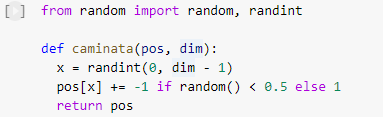
\includegraphics[scale=0.7]{Caminata.png}
    \caption{Caminata del movimiento Browniano}
    \label{fig:f1}
\end{figure}
     
\section{Resultados obtenidos}
Repetidas las pruebas para todas las dimensiones y para todos los pasos de la caminata, se obtuvieron valores del porcentaje de la cantidad de veces que retornaba al origen la partícula en las diferentes pruebas; datos con los que fue elaborado una matrix para analizar su comportamiento. El comportamiento de la partícula para todas las pruebas hechas se observa en un diagrama de caja-bigote(Figura 2), cuyo eje $x$ está representado por las dimensiones y el eje $y$ por el porcentaje obtenido de regreso de la partícula al origen. Como se observa en el comportamiento, se hace más difícil a la partícula regresar al  aumentar las dimensiones.  

\begin{figure}[H]
    \centering

    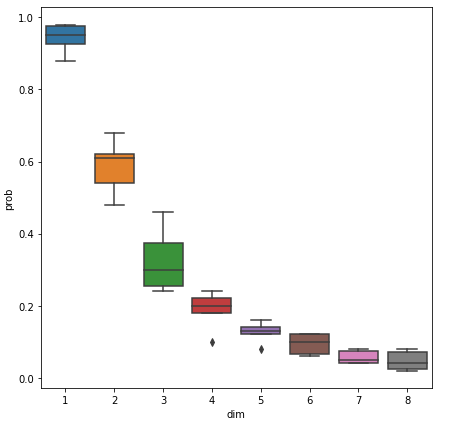
\includegraphics[scale=0.7]{Caja.png}
    \caption{Diagrama de caja-bigote para 8 dimensiones}
    \label{fig:f2}
\end{figure}

A continuación se muestra también de los datos recogidos, un cuadro indicando el mínimo, promedio y máximo del tiempo de regreso (en porciento).
\begin{center}
\begin{tabular}{|c|c|c|c|}
\hline 
Dimensión & Mínimo & Promedio & Máximo \\ 
\hline 
1 & 0.88 & 0.94 & 0.98 \\ 
\hline 
2 & 0.48 & 0.6 & 0.68 \\ 
\hline 
3 & 0.24 & 0.3 & 0.48 \\ 
\hline 
4 & 0.1 & 0.18 & 0.24 \\ 
\hline 
5 & 0.08 & 0.12 & 0.14 \\ 
\hline 
6 & 0.06 & 0.09 & 0.12 \\ 
\hline 
7 & 0.04 & 0.06 & 0.08 \\ 
\hline 
8 & 0.02 & 0.04 & 0.08 \\ 
\hline 
\end{tabular} 
\end{center}

\section{Conclusiones}
Se puede concluir con los experimentos realizados que se hace más complejo el regreso de la partícula mientras aumentan las dimensiones, por el contrario se hace más estable el experimento al aumentar los pasos. Este análisis fue realizado para la caminata manhattan, es necesario continuar trabajando y realizar pruebas para la euclediana, además de hacer un mayor número de pruebas para lograr ver bien el comportamiento en fracciones de tiempo pequeñas. 
\end{document} 
